% Options for packages loaded elsewhere
% Options for packages loaded elsewhere
\PassOptionsToPackage{unicode}{hyperref}
\PassOptionsToPackage{hyphens}{url}
\PassOptionsToPackage{dvipsnames,svgnames,x11names}{xcolor}
%
\documentclass[
  letterpaper,
  DIV=11,
  numbers=noendperiod]{scrartcl}
\usepackage{xcolor}
\usepackage{amsmath,amssymb}
\setcounter{secnumdepth}{5}
\usepackage{iftex}
\ifPDFTeX
  \usepackage[T1]{fontenc}
  \usepackage[utf8]{inputenc}
  \usepackage{textcomp} % provide euro and other symbols
\else % if luatex or xetex
  \usepackage{unicode-math} % this also loads fontspec
  \defaultfontfeatures{Scale=MatchLowercase}
  \defaultfontfeatures[\rmfamily]{Ligatures=TeX,Scale=1}
\fi
\usepackage{lmodern}
\ifPDFTeX\else
  % xetex/luatex font selection
\fi
% Use upquote if available, for straight quotes in verbatim environments
\IfFileExists{upquote.sty}{\usepackage{upquote}}{}
\IfFileExists{microtype.sty}{% use microtype if available
  \usepackage[]{microtype}
  \UseMicrotypeSet[protrusion]{basicmath} % disable protrusion for tt fonts
}{}
\makeatletter
\@ifundefined{KOMAClassName}{% if non-KOMA class
  \IfFileExists{parskip.sty}{%
    \usepackage{parskip}
  }{% else
    \setlength{\parindent}{0pt}
    \setlength{\parskip}{6pt plus 2pt minus 1pt}}
}{% if KOMA class
  \KOMAoptions{parskip=half}}
\makeatother
% Make \paragraph and \subparagraph free-standing
\makeatletter
\ifx\paragraph\undefined\else
  \let\oldparagraph\paragraph
  \renewcommand{\paragraph}{
    \@ifstar
      \xxxParagraphStar
      \xxxParagraphNoStar
  }
  \newcommand{\xxxParagraphStar}[1]{\oldparagraph*{#1}\mbox{}}
  \newcommand{\xxxParagraphNoStar}[1]{\oldparagraph{#1}\mbox{}}
\fi
\ifx\subparagraph\undefined\else
  \let\oldsubparagraph\subparagraph
  \renewcommand{\subparagraph}{
    \@ifstar
      \xxxSubParagraphStar
      \xxxSubParagraphNoStar
  }
  \newcommand{\xxxSubParagraphStar}[1]{\oldsubparagraph*{#1}\mbox{}}
  \newcommand{\xxxSubParagraphNoStar}[1]{\oldsubparagraph{#1}\mbox{}}
\fi
\makeatother

\usepackage{color}
\usepackage{fancyvrb}
\newcommand{\VerbBar}{|}
\newcommand{\VERB}{\Verb[commandchars=\\\{\}]}
\DefineVerbatimEnvironment{Highlighting}{Verbatim}{commandchars=\\\{\}}
% Add ',fontsize=\small' for more characters per line
\usepackage{framed}
\definecolor{shadecolor}{RGB}{241,243,245}
\newenvironment{Shaded}{\begin{snugshade}}{\end{snugshade}}
\newcommand{\AlertTok}[1]{\textcolor[rgb]{0.68,0.00,0.00}{#1}}
\newcommand{\AnnotationTok}[1]{\textcolor[rgb]{0.37,0.37,0.37}{#1}}
\newcommand{\AttributeTok}[1]{\textcolor[rgb]{0.40,0.45,0.13}{#1}}
\newcommand{\BaseNTok}[1]{\textcolor[rgb]{0.68,0.00,0.00}{#1}}
\newcommand{\BuiltInTok}[1]{\textcolor[rgb]{0.00,0.23,0.31}{#1}}
\newcommand{\CharTok}[1]{\textcolor[rgb]{0.13,0.47,0.30}{#1}}
\newcommand{\CommentTok}[1]{\textcolor[rgb]{0.37,0.37,0.37}{#1}}
\newcommand{\CommentVarTok}[1]{\textcolor[rgb]{0.37,0.37,0.37}{\textit{#1}}}
\newcommand{\ConstantTok}[1]{\textcolor[rgb]{0.56,0.35,0.01}{#1}}
\newcommand{\ControlFlowTok}[1]{\textcolor[rgb]{0.00,0.23,0.31}{\textbf{#1}}}
\newcommand{\DataTypeTok}[1]{\textcolor[rgb]{0.68,0.00,0.00}{#1}}
\newcommand{\DecValTok}[1]{\textcolor[rgb]{0.68,0.00,0.00}{#1}}
\newcommand{\DocumentationTok}[1]{\textcolor[rgb]{0.37,0.37,0.37}{\textit{#1}}}
\newcommand{\ErrorTok}[1]{\textcolor[rgb]{0.68,0.00,0.00}{#1}}
\newcommand{\ExtensionTok}[1]{\textcolor[rgb]{0.00,0.23,0.31}{#1}}
\newcommand{\FloatTok}[1]{\textcolor[rgb]{0.68,0.00,0.00}{#1}}
\newcommand{\FunctionTok}[1]{\textcolor[rgb]{0.28,0.35,0.67}{#1}}
\newcommand{\ImportTok}[1]{\textcolor[rgb]{0.00,0.46,0.62}{#1}}
\newcommand{\InformationTok}[1]{\textcolor[rgb]{0.37,0.37,0.37}{#1}}
\newcommand{\KeywordTok}[1]{\textcolor[rgb]{0.00,0.23,0.31}{\textbf{#1}}}
\newcommand{\NormalTok}[1]{\textcolor[rgb]{0.00,0.23,0.31}{#1}}
\newcommand{\OperatorTok}[1]{\textcolor[rgb]{0.37,0.37,0.37}{#1}}
\newcommand{\OtherTok}[1]{\textcolor[rgb]{0.00,0.23,0.31}{#1}}
\newcommand{\PreprocessorTok}[1]{\textcolor[rgb]{0.68,0.00,0.00}{#1}}
\newcommand{\RegionMarkerTok}[1]{\textcolor[rgb]{0.00,0.23,0.31}{#1}}
\newcommand{\SpecialCharTok}[1]{\textcolor[rgb]{0.37,0.37,0.37}{#1}}
\newcommand{\SpecialStringTok}[1]{\textcolor[rgb]{0.13,0.47,0.30}{#1}}
\newcommand{\StringTok}[1]{\textcolor[rgb]{0.13,0.47,0.30}{#1}}
\newcommand{\VariableTok}[1]{\textcolor[rgb]{0.07,0.07,0.07}{#1}}
\newcommand{\VerbatimStringTok}[1]{\textcolor[rgb]{0.13,0.47,0.30}{#1}}
\newcommand{\WarningTok}[1]{\textcolor[rgb]{0.37,0.37,0.37}{\textit{#1}}}

\usepackage{longtable,booktabs,array}
\usepackage{calc} % for calculating minipage widths
% Correct order of tables after \paragraph or \subparagraph
\usepackage{etoolbox}
\makeatletter
\patchcmd\longtable{\par}{\if@noskipsec\mbox{}\fi\par}{}{}
\makeatother
% Allow footnotes in longtable head/foot
\IfFileExists{footnotehyper.sty}{\usepackage{footnotehyper}}{\usepackage{footnote}}
\makesavenoteenv{longtable}
\usepackage{graphicx}
\makeatletter
\newsavebox\pandoc@box
\newcommand*\pandocbounded[1]{% scales image to fit in text height/width
  \sbox\pandoc@box{#1}%
  \Gscale@div\@tempa{\textheight}{\dimexpr\ht\pandoc@box+\dp\pandoc@box\relax}%
  \Gscale@div\@tempb{\linewidth}{\wd\pandoc@box}%
  \ifdim\@tempb\p@<\@tempa\p@\let\@tempa\@tempb\fi% select the smaller of both
  \ifdim\@tempa\p@<\p@\scalebox{\@tempa}{\usebox\pandoc@box}%
  \else\usebox{\pandoc@box}%
  \fi%
}
% Set default figure placement to htbp
\def\fps@figure{htbp}
\makeatother

\ifLuaTeX
  \usepackage{luacolor}
  \usepackage[soul]{lua-ul}
\else
  \usepackage{soul}
\fi




\setlength{\emergencystretch}{3em} % prevent overfull lines

\providecommand{\tightlist}{%
  \setlength{\itemsep}{0pt}\setlength{\parskip}{0pt}}



 


\KOMAoption{captions}{tableheading}
\makeatletter
\@ifpackageloaded{caption}{}{\usepackage{caption}}
\AtBeginDocument{%
\ifdefined\contentsname
  \renewcommand*\contentsname{Table of contents}
\else
  \newcommand\contentsname{Table of contents}
\fi
\ifdefined\listfigurename
  \renewcommand*\listfigurename{List of Figures}
\else
  \newcommand\listfigurename{List of Figures}
\fi
\ifdefined\listtablename
  \renewcommand*\listtablename{List of Tables}
\else
  \newcommand\listtablename{List of Tables}
\fi
\ifdefined\figurename
  \renewcommand*\figurename{Figure}
\else
  \newcommand\figurename{Figure}
\fi
\ifdefined\tablename
  \renewcommand*\tablename{Table}
\else
  \newcommand\tablename{Table}
\fi
}
\@ifpackageloaded{float}{}{\usepackage{float}}
\floatstyle{ruled}
\@ifundefined{c@chapter}{\newfloat{codelisting}{h}{lop}}{\newfloat{codelisting}{h}{lop}[chapter]}
\floatname{codelisting}{Listing}
\newcommand*\listoflistings{\listof{codelisting}{List of Listings}}
\makeatother
\makeatletter
\makeatother
\makeatletter
\@ifpackageloaded{caption}{}{\usepackage{caption}}
\@ifpackageloaded{subcaption}{}{\usepackage{subcaption}}
\makeatother
\usepackage{bookmark}
\IfFileExists{xurl.sty}{\usepackage{xurl}}{} % add URL line breaks if available
\urlstyle{same}
\hypersetup{
  pdftitle={descriptives},
  colorlinks=true,
  linkcolor={blue},
  filecolor={Maroon},
  citecolor={Blue},
  urlcolor={Blue},
  pdfcreator={LaTeX via pandoc}}


\title{descriptives}
\author{}
\date{}
\begin{document}
\maketitle

\renewcommand*\contentsname{Table of contents}
{
\hypersetup{linkcolor=}
\setcounter{tocdepth}{3}
\tableofcontents
}

\begin{Shaded}
\begin{Highlighting}[]
\NormalTok{starwars }\OtherTok{\textless{}{-}}\NormalTok{ dplyr}\SpecialCharTok{::}\NormalTok{starwars}
\end{Highlighting}
\end{Shaded}

\begin{Shaded}
\begin{Highlighting}[]
\FunctionTok{names}\NormalTok{(starwars)}
\end{Highlighting}
\end{Shaded}

\begin{verbatim}
 [1] "name"       "height"     "mass"       "hair_color" "skin_color"
 [6] "eye_color"  "birth_year" "sex"        "gender"     "homeworld" 
[11] "species"    "films"      "vehicles"   "starships" 
\end{verbatim}

\begin{Shaded}
\begin{Highlighting}[]
\FunctionTok{glimpse}\NormalTok{(starwars)}
\end{Highlighting}
\end{Shaded}

\begin{verbatim}
Rows: 87
Columns: 14
$ name       <chr> "Luke Skywalker", "C-3PO", "R2-D2", "Darth Vader", "Leia Or~
$ height     <int> 172, 167, 96, 202, 150, 178, 165, 97, 183, 182, 188, 180, 2~
$ mass       <dbl> 77.0, 75.0, 32.0, 136.0, 49.0, 120.0, 75.0, 32.0, 84.0, 77.~
$ hair_color <chr> "blond", NA, NA, "none", "brown", "brown, grey", "brown", N~
$ skin_color <chr> "fair", "gold", "white, blue", "white", "light", "light", "~
$ eye_color  <chr> "blue", "yellow", "red", "yellow", "brown", "blue", "blue",~
$ birth_year <dbl> 19.0, 112.0, 33.0, 41.9, 19.0, 52.0, 47.0, NA, 24.0, 57.0, ~
$ sex        <chr> "male", "none", "none", "male", "female", "male", "female",~
$ gender     <chr> "masculine", "masculine", "masculine", "masculine", "femini~
$ homeworld  <chr> "Tatooine", "Tatooine", "Naboo", "Tatooine", "Alderaan", "T~
$ species    <chr> "Human", "Droid", "Droid", "Human", "Human", "Human", "Huma~
$ films      <list> <"A New Hope", "The Empire Strikes Back", "Return of the J~
$ vehicles   <list> <"Snowspeeder", "Imperial Speeder Bike">, <>, <>, <>, "Imp~
$ starships  <list> <"X-wing", "Imperial shuttle">, <>, <>, "TIE Advanced x1",~
\end{verbatim}

\section{Descriptive Statistics}\label{descriptive-statistics}

\begin{longtable}[]{@{}ll@{}}
\toprule\noalign{}
\ul{P}opulation & \ul{S}ample \\
\midrule\noalign{}
\endhead
\bottomrule\noalign{}
\endlastfoot
\ul{P}arameters & \ul{S}tatistics \\
\end{longtable}

\subsection{Location / Central
Tendency}\label{location-central-tendency}

\subsubsection{Mode}\label{mode}

The mode of a sample is very simple: it is the value that occurs
\textbf{most frequently}.~

A frequency table could be examined.

\begin{Shaded}
\begin{Highlighting}[]
\NormalTok{descr}\SpecialCharTok{::}\FunctionTok{freq}\NormalTok{(}\FunctionTok{as.ordered}\NormalTok{(starwars}\SpecialCharTok{$}\NormalTok{eye\_color), }\AttributeTok{plot =} \ConstantTok{FALSE}\NormalTok{)}
\end{Highlighting}
\end{Shaded}

\begin{verbatim}
as.ordered(starwars$eye_color) 
              Frequency Percent Cum Percent
black                10  11.494       11.49
blue                 19  21.839       33.33
blue-gray             1   1.149       34.48
brown                21  24.138       58.62
dark                  1   1.149       59.77
gold                  1   1.149       60.92
green, yellow         1   1.149       62.07
hazel                 3   3.448       65.52
orange                8   9.195       74.71
pink                  1   1.149       75.86
red                   5   5.747       81.61
red, blue             1   1.149       82.76
unknown               3   3.448       86.21
white                 1   1.149       87.36
yellow               11  12.644      100.00
Total                87 100.000            
\end{verbatim}

\begin{Shaded}
\begin{Highlighting}[]
\FunctionTok{modeOf}\NormalTok{(}\AttributeTok{x =}\NormalTok{ starwars}\SpecialCharTok{$}\NormalTok{eye\_color)}
\end{Highlighting}
\end{Shaded}

\begin{verbatim}
[1] "brown"
\end{verbatim}

\paragraph{No Mode = same frequency}\label{no-mode-same-frequency}

\begin{Shaded}
\begin{Highlighting}[]
\NormalTok{y }\OtherTok{=} \DecValTok{100}

\FunctionTok{ggplot}\NormalTok{() }\SpecialCharTok{+}
  \FunctionTok{geom\_hline}\NormalTok{(}\AttributeTok{yintercept =}\NormalTok{ y)}
\end{Highlighting}
\end{Shaded}

\pandocbounded{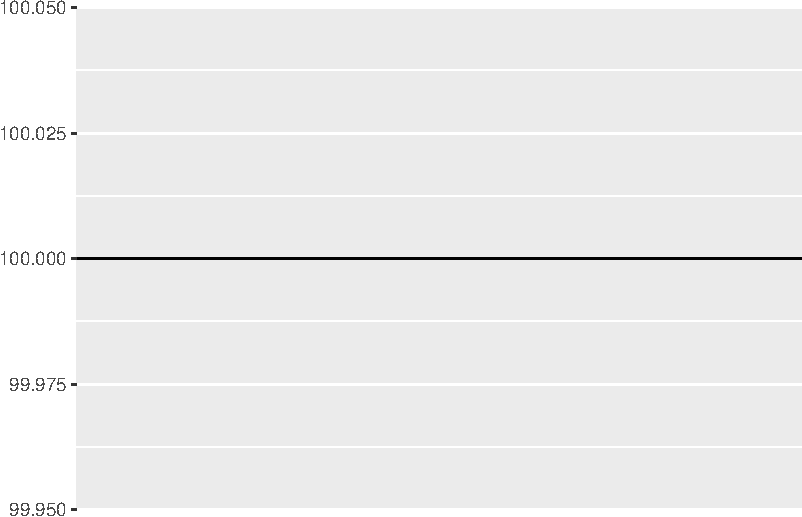
\includegraphics[keepaspectratio]{descriptives_files/figure-pdf/unnamed-chunk-7-1.pdf}}

\paragraph{Bimodal = two modes}\label{bimodal-two-modes}

\begin{Shaded}
\begin{Highlighting}[]
\CommentTok{\# Create data}
\FunctionTok{set.seed}\NormalTok{(}\DecValTok{123}\NormalTok{)}

\NormalTok{n }\OtherTok{\textless{}{-}} \DecValTok{1000} \CommentTok{\# Sample split in each below}

\NormalTok{x }\OtherTok{\textless{}{-}} \FunctionTok{c}\NormalTok{(}
  \FunctionTok{rnorm}\NormalTok{(n }\SpecialCharTok{/} \DecValTok{2}\NormalTok{, }\AttributeTok{mean =} \DecValTok{0}\NormalTok{, }\AttributeTok{sd =} \DecValTok{1}\NormalTok{), }\CommentTok{\# Update mean or sd}
  \FunctionTok{rnorm}\NormalTok{(n }\SpecialCharTok{/} \DecValTok{2}\NormalTok{, }\AttributeTok{mean =} \DecValTok{3}\NormalTok{, }\AttributeTok{sd =} \DecValTok{1}\NormalTok{)}
\NormalTok{)}

\NormalTok{df }\OtherTok{\textless{}{-}} \FunctionTok{data.frame}\NormalTok{(x)}

\CommentTok{\# Visualize}
\FunctionTok{ggplot}\NormalTok{(df, }\FunctionTok{aes}\NormalTok{(x)) }\SpecialCharTok{+}
  \FunctionTok{geom\_histogram}\NormalTok{(}\AttributeTok{bins =} \DecValTok{40}\NormalTok{)}
\end{Highlighting}
\end{Shaded}

\pandocbounded{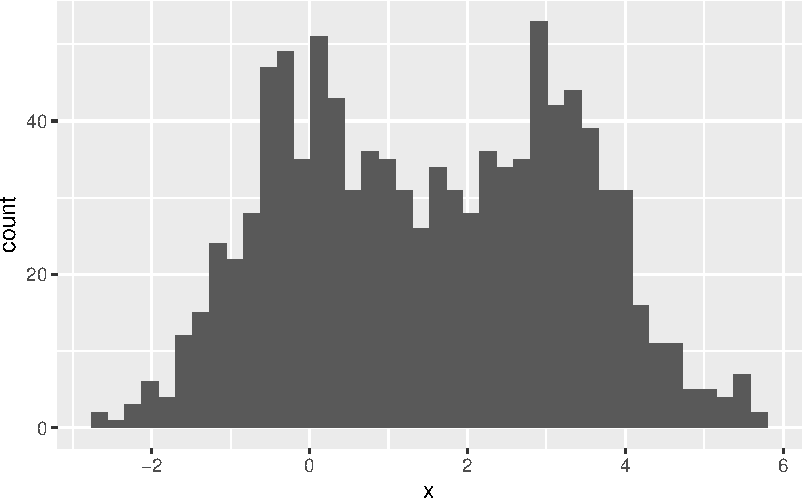
\includegraphics[keepaspectratio]{descriptives_files/figure-pdf/unnamed-chunk-8-1.pdf}}

\paragraph{Multimodal = \textgreater2 modes}\label{multimodal-2-modes}

\begin{Shaded}
\begin{Highlighting}[]
\CommentTok{\# Create data}
\FunctionTok{set.seed}\NormalTok{(}\DecValTok{123}\NormalTok{)}

\NormalTok{n }\OtherTok{\textless{}{-}} \DecValTok{1500} \CommentTok{\# Sample split in each below}

\NormalTok{x }\OtherTok{\textless{}{-}} \FunctionTok{c}\NormalTok{(}
  \FunctionTok{rnorm}\NormalTok{(n }\SpecialCharTok{/} \DecValTok{3}\NormalTok{, }\AttributeTok{mean =} \DecValTok{0}\NormalTok{, }\AttributeTok{sd =} \DecValTok{1}\NormalTok{), }\CommentTok{\# Update mean or sd}
  \FunctionTok{rnorm}\NormalTok{(n }\SpecialCharTok{/} \DecValTok{3}\NormalTok{, }\AttributeTok{mean =} \DecValTok{3}\NormalTok{, }\AttributeTok{sd =} \DecValTok{1}\NormalTok{),}
  \FunctionTok{rnorm}\NormalTok{(n }\SpecialCharTok{/} \DecValTok{3}\NormalTok{, }\AttributeTok{mean =} \DecValTok{6}\NormalTok{, }\AttributeTok{sd =} \DecValTok{1}\NormalTok{)}
\NormalTok{)}

\NormalTok{df }\OtherTok{\textless{}{-}} \FunctionTok{data.frame}\NormalTok{(x)}

\CommentTok{\# Visualize}
\FunctionTok{ggplot}\NormalTok{(df, }\FunctionTok{aes}\NormalTok{(x)) }\SpecialCharTok{+}
  \FunctionTok{geom\_histogram}\NormalTok{(}\AttributeTok{bins =} \DecValTok{40}\NormalTok{)}
\end{Highlighting}
\end{Shaded}

\pandocbounded{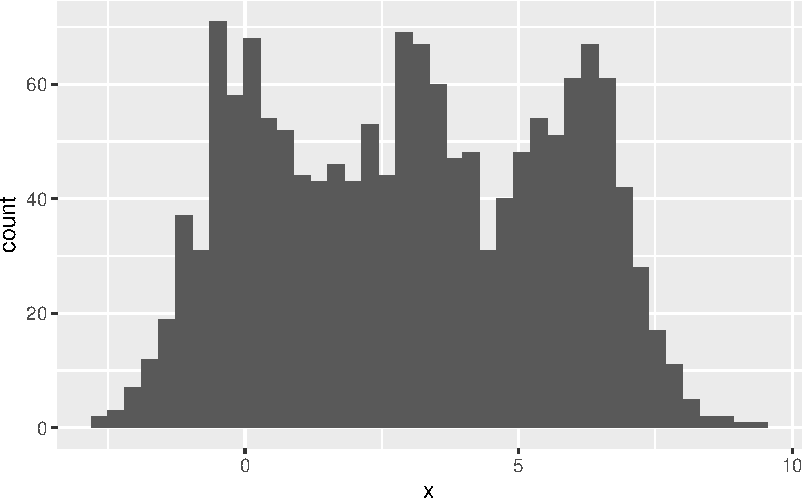
\includegraphics[keepaspectratio]{descriptives_files/figure-pdf/unnamed-chunk-9-1.pdf}}

\subsubsection{Median}\label{median}

The median of a set of observations is just the \textbf{middle value}.
Let's imagine we were interested only in the first 5 AFL winning
margins. To figure out the median, we sort these numbers into ascending
order:

\[8, 31,\mathbf{32},56,56 \]

From inspection, it's obvious that the median value of these 5
observations is 32, since that's the middle one in the sorted list (I've
put it in bold to make it even more obvious). Easy stuff.

But what should we do if we were interested in the first 6 games rather
than the first 5? Since the sixth game in the season had a winning
margin of 14 points, our sorted list is now.

\[8,14,\mathbf{31,32},56,56\]

and there are~\emph{two}~middle numbers, 31 and 32. The median is
defined as the average of those two numbers, which is of course 31.5.~

As before, it's very tedious to do this by hand when you've got lots of
numbers.~In real life, of course, no-one actually calculates the median
by sorting the data and then looking for the middle value. In real life,
we use the median command:

\begin{Shaded}
\begin{Highlighting}[]
\FunctionTok{median}\NormalTok{(starwars}\SpecialCharTok{$}\NormalTok{mass, }\AttributeTok{na.rm =} \ConstantTok{TRUE}\NormalTok{)}
\end{Highlighting}
\end{Shaded}

\begin{verbatim}
[1] 79
\end{verbatim}

\begin{Shaded}
\begin{Highlighting}[]
\CommentTok{\# If you variable contains even one NA, this function will return NA, unless you tell it to ignore the NAs. }
\end{Highlighting}
\end{Shaded}

\subsubsection{Arithmetic Mean}\label{arithmetic-mean}

\emph{Typical, old-fashioned average. Add all of the values up, and then
divide by the total number of values.}

\[\frac{1}{n}\left(x_1 + x_2 + \cdots + x_n\right)\]

where \(x_i, x_2 \ldots x_n\) are the observed values and \(n\) is the
number of observations.

\begin{longtable}[]{@{}
  >{\raggedright\arraybackslash}p{(\linewidth - 2\tabcolsep) * \real{0.5211}}
  >{\raggedright\arraybackslash}p{(\linewidth - 2\tabcolsep) * \real{0.4789}}@{}}
\toprule\noalign{}
\begin{minipage}[b]{\linewidth}\raggedright
Population
\end{minipage} & \begin{minipage}[b]{\linewidth}\raggedright
Sample
\end{minipage} \\
\midrule\noalign{}
\endhead
\bottomrule\noalign{}
\endlastfoot
\(                     
 \mu = \frac{\sum y}{N}  
 \) & \(                   
                          m = \frac{\sum y}{n}  
                          \) \\
\end{longtable}

For example, for the values 56, 31, 56, 8, 32:

\[\bar{x} = \frac{x_1 + x_2 + x_3 + \cdots + x_n}{n}\]

\[\bar{x} = \frac{56 + 31 + 56 + 8 + 32}{5}\]

\[\bar{x} = \frac{183}{5} = 36.60\]

Written out:

\begin{Shaded}
\begin{Highlighting}[]
\NormalTok{(}\DecValTok{56} \SpecialCharTok{+} \DecValTok{31} \SpecialCharTok{+} \DecValTok{56} \SpecialCharTok{+} \DecValTok{8} \SpecialCharTok{+} \DecValTok{32}\NormalTok{) }\SpecialCharTok{/} \DecValTok{5}
\end{Highlighting}
\end{Shaded}

\begin{verbatim}
[1] 36.6
\end{verbatim}

We can tell R to same thing with functions.

\begin{Shaded}
\begin{Highlighting}[]
\NormalTok{x }\OtherTok{\textless{}{-}} \FunctionTok{c}\NormalTok{(}\DecValTok{56}\NormalTok{, }\DecValTok{31}\NormalTok{, }\DecValTok{56}\NormalTok{, }\DecValTok{8}\NormalTok{, }\DecValTok{32}\NormalTok{)}
\FunctionTok{sum}\NormalTok{(x) }\SpecialCharTok{/} \FunctionTok{length}\NormalTok{(x)}
\end{Highlighting}
\end{Shaded}

\begin{verbatim}
[1] 36.6
\end{verbatim}

Although it's pretty easy to calculate the mean using
the~\texttt{sum()}~function, we can do it in an even easier way, since R
also provides us with the~\texttt{mean()}~function.

\begin{Shaded}
\begin{Highlighting}[]
\NormalTok{x }\OtherTok{\textless{}{-}} \FunctionTok{c}\NormalTok{(}\DecValTok{56}\NormalTok{, }\DecValTok{31}\NormalTok{, }\DecValTok{56}\NormalTok{, }\DecValTok{8}\NormalTok{, }\DecValTok{32}\NormalTok{)}
\FunctionTok{mean}\NormalTok{(x, }\AttributeTok{na.rm =} \ConstantTok{TRUE}\NormalTok{)}
\end{Highlighting}
\end{Shaded}

\begin{verbatim}
[1] 36.6
\end{verbatim}

\paragraph{Which one? Median vs Mean}\label{which-one-median-vs-mean}

Knowing how to calculate means and medians is only a part of the story.
You also need to understand what each one is saying about the data, and
what that implies for when you should use each one.~

\pandocbounded{\includegraphics[keepaspectratio]{images/clipboard-3927156023.png}}

The mean is kind of like the ``centre of gravity'' of the data set,
whereas the median is the ``middle value'' in the data.~What this
implies, as far as which one you should use, depends a little on what
type of data you've got and what you're trying to achieve. As a rough
guide:

\begin{itemize}
\item
  \textbf{Nominal data:} Use the mode.
\item
  \textbf{Ordinal data:} More likely to want to use the median than the
  mean. The median only makes use of the order information in your data
  (i.e., which numbers are bigger), but doesn't depend on the precise
  numbers involved. That's exactly the situation that applies when your
  data are ordinal scale. The mean, on the other hand, makes use of the
  precise numeric values assigned to the observations, so it's not
  really appropriate for ordinal data.
\item
  \textbf{Interval} and \textbf{Ratio} scale data: either mean or median
  is generally acceptable. Which one you pick depends a bit on what
  you're trying to achieve. The mean has the advantage that it uses all
  the information in the data (which is useful when you don't have a lot
  of data), but it's very sensitive to extreme values.
\end{itemize}

\begin{center}\rule{0.5\linewidth}{0.5pt}\end{center}

\subsubsection{Weighted Mean}\label{weighted-mean}

\emph{An average where some of the values count more than others.
Instead of treating every value equally, each value is multiplied by an
assigned weight.}

Computed by multiplying each observation by its corresponding weight,
summing those products, and dividing by the sum of the weights.

\[\bar{x}= \frac{w_1 x_1 + w_2 x_2 + \cdots + w_n x_n}       {w_1 + w_2 + \cdots + w_n}= \frac{\sum w_i x_i}{\sum w_i}\]

where \(x_i\) is the i-th observation and \(w_i\) is its corresponding
weight.

\begin{Shaded}
\begin{Highlighting}[]
\NormalTok{x }\OtherTok{\textless{}{-}} \FunctionTok{c}\NormalTok{(}\DecValTok{70}\NormalTok{, }\DecValTok{80}\NormalTok{, }\DecValTok{90}\NormalTok{) }\CommentTok{\# observations}
\NormalTok{w }\OtherTok{\textless{}{-}} \FunctionTok{c}\NormalTok{(}\DecValTok{50}\NormalTok{, }\DecValTok{40}\NormalTok{, }\DecValTok{10}\NormalTok{)  }\CommentTok{\# weights}

\FunctionTok{sum}\NormalTok{(x }\SpecialCharTok{*}\NormalTok{ w) }\SpecialCharTok{/} \FunctionTok{sum}\NormalTok{(w)}
\end{Highlighting}
\end{Shaded}

\begin{verbatim}
[1] 76
\end{verbatim}

R has build-in function for this.

\begin{Shaded}
\begin{Highlighting}[]
\FunctionTok{weighted.mean}\NormalTok{(x, w)}
\end{Highlighting}
\end{Shaded}

\begin{verbatim}
[1] 76
\end{verbatim}

\subsubsection{Trimmed Mean}\label{trimmed-mean}

\emph{Discards a percentage of extreme values from both ends and
calculates the mean}

\[\bar{x}_{\text{trim}} =\frac{x_{(k+1)} + x_{(k+2)} + \cdots + x_{(n-k)}}{n - 2k}\]

where \(x_{(i)}\) denotes the i-th ordered observation and \(k\) is the
number of values trimmed from each tail.

For example, consider this strange looking data set:

\[ -100, 2, 3, 4, 5, 6, 7, 8, 9, 10 \]

If you were to observe this in a real life data set, you'd probably
suspect that something funny was going on with the~−100~value. It's
probably an~\textbf{\emph{outlier}}, a value that doesn't really belong
with the others. You might consider removing it from the data set
entirely, and in this particular case I'd probably agree with that
course of action. In real life, however, you don't always get such
cut-and-dried examples. For instance, you might get this instead:\\
\[ −15,2,3,4,5,6,7,8,9,12 \]

The~−15~looks a bit suspicious, but not anywhere near as much as
that~−100~did. In this case, it's a little trickier. It~\emph{might}~be
a legitimate observation, it might not.

When faced with a situation where some of the most extreme-valued
observations might not be quite trustworthy, the mean is not necessarily
a good measure of central tendency. It is highly sensitive to one or two
extreme values, and is thus not considered to be
a~\textbf{\emph{robust}}~measure.~

One remedy that we've seen is to use the median. A more general solution
is to use a ``trimmed mean''.~

To calculate a trimmed mean, what you do is ``discard'' the most extreme
examples on both ends (i.e., the largest and the smallest), and then
take the mean of everything else. The goal is to preserve the best
characteristics of the mean and the median: just like a median, you
aren't highly influenced by extreme outliers, but like the mean, you
``use'' more than one of the observations.~

Generally, we describe a trimmed mean in terms of the percentage of
observation on either side that are discarded. So, for instance, a 10\%
trimmed mean discards the largest 10\% of the observations \emph{and}
the smallest 10\% of the observations, and then takes the mean of the
remaining 80\% of the observations. Not surprisingly, the 0\% trimmed
mean is just the regular mean, and the 50\% trimmed mean is the median.
In that sense, trimmed means provide a whole family of central tendency
measures that span the range from the mean to the median.

For our toy example above, we have 10 observations, and so a 10\%
trimmed mean is calculated by ignoring the largest value (i.e.,
\texttt{12}) and the smallest value (i.e., \texttt{-15}) and taking the
mean of the remaining values.

First, let's enter the data.

\begin{Shaded}
\begin{Highlighting}[]
\NormalTok{x }\OtherTok{\textless{}{-}} \FunctionTok{c}\NormalTok{(}\SpecialCharTok{{-}}\DecValTok{15}\NormalTok{,}\DecValTok{2}\NormalTok{,}\DecValTok{3}\NormalTok{,}\DecValTok{4}\NormalTok{,}\DecValTok{5}\NormalTok{,}\DecValTok{6}\NormalTok{,}\DecValTok{7}\NormalTok{,}\DecValTok{8}\NormalTok{,}\DecValTok{9}\NormalTok{,}\DecValTok{12}\NormalTok{)}
\end{Highlighting}
\end{Shaded}

Next, let's calculate means and medians:

\begin{Shaded}
\begin{Highlighting}[]
\FunctionTok{mean}\NormalTok{(x)}
\end{Highlighting}
\end{Shaded}

\begin{verbatim}
[1] 4.1
\end{verbatim}

\begin{Shaded}
\begin{Highlighting}[]
\FunctionTok{median}\NormalTok{(x)}
\end{Highlighting}
\end{Shaded}

\begin{verbatim}
[1] 5.5
\end{verbatim}

That's a fairly substantial difference, but I'm tempted to think that
the mean is being influenced a bit too much by the extreme values at
either end of the data set, especially the~−15~one. So let's just try
trimming the mean a bit. If I take a 10\% trimmed mean, we'll drop the
extreme values on either side, and take the mean of the rest:

\begin{Shaded}
\begin{Highlighting}[]
\FunctionTok{mean}\NormalTok{(x, }\AttributeTok{trim =}\NormalTok{ .}\DecValTok{1}\NormalTok{)}
\end{Highlighting}
\end{Shaded}

\begin{verbatim}
[1] 5.5
\end{verbatim}

which in this case gives exactly the same answer as the median. Note
that, to get a 10\% trimmed mean you write~\texttt{trim\ =\ .1},
not~\texttt{trim\ =\ 10}.

\begin{center}\rule{0.5\linewidth}{0.5pt}\end{center}

\subsection{Skew and Kurtosis}\label{skew-and-kurtosis}

There are two more descriptive statistics that you will sometimes see
reported in the psychological literature, known as skew and kurtosis. In
practice, neither one is used anywhere near as frequently as the
measures of central tendency and variability that we've been talking
about.

Skew is pretty important, so you do see it mentioned a fair bit; but
I've actually never seen kurtosis reported in a scientific article to
date.

\subsubsection{Skew}\label{skew}

Since it's the more interesting of the two, let's start by talking about
the~\textbf{\emph{skewness}}. Skewness is basically a measure of
asymmetry, and the easiest way to explain it is by drawing some
pictures.~

Right skew or positively skewed: Tail on the right.

Left skew or negatively skewed: Tail on the left.

\begin{Shaded}
\begin{Highlighting}[]
\FunctionTok{set.seed}\NormalTok{(}\DecValTok{123}\NormalTok{)}

\NormalTok{n }\OtherTok{\textless{}{-}} \DecValTok{1000}

\CommentTok{\# Positive skew: Gamma (right tail)}
\NormalTok{pos }\OtherTok{\textless{}{-}} \FunctionTok{rgamma}\NormalTok{(n, }\AttributeTok{shape =} \DecValTok{6}\NormalTok{, }\AttributeTok{scale =} \DecValTok{1}\NormalTok{)}

\CommentTok{\# No skew: Normal}
\NormalTok{noskew }\OtherTok{\textless{}{-}} \FunctionTok{rnorm}\NormalTok{(n, }\AttributeTok{mean =} \FunctionTok{mean}\NormalTok{(pos), }\AttributeTok{sd =} \FunctionTok{sd}\NormalTok{(pos))}

\CommentTok{\# Negative skew: reflect the positive skew around its max (left tail)}
\NormalTok{neg }\OtherTok{\textless{}{-}} \FunctionTok{max}\NormalTok{(pos) }\SpecialCharTok{{-}}\NormalTok{ pos}

\NormalTok{df }\OtherTok{\textless{}{-}} \FunctionTok{bind\_rows}\NormalTok{(}
  \FunctionTok{tibble}\NormalTok{(}\AttributeTok{x =}\NormalTok{ neg,    }\AttributeTok{skew =} \StringTok{"Negative Skew"}\NormalTok{),}
  \FunctionTok{tibble}\NormalTok{(}\AttributeTok{x =}\NormalTok{ noskew, }\AttributeTok{skew =} \StringTok{"No Skew"}\NormalTok{),}
  \FunctionTok{tibble}\NormalTok{(}\AttributeTok{x =}\NormalTok{ pos,    }\AttributeTok{skew =} \StringTok{"Positive Skew"}\NormalTok{)}
\NormalTok{)}

\FunctionTok{ggplot}\NormalTok{(df, }\FunctionTok{aes}\NormalTok{(x)) }\SpecialCharTok{+}
  \FunctionTok{geom\_histogram}\NormalTok{(}\AttributeTok{bins =} \DecValTok{20}\NormalTok{, }\AttributeTok{fill =} \StringTok{"cornflowerblue"}\NormalTok{, }\AttributeTok{color =} \StringTok{"white"}\NormalTok{) }\SpecialCharTok{+}
  \FunctionTok{facet\_wrap}\NormalTok{(}\SpecialCharTok{\textasciitilde{}}\NormalTok{ skew, }\AttributeTok{nrow =} \DecValTok{1}\NormalTok{, }\AttributeTok{scales =} \StringTok{"free\_x"}\NormalTok{) }\SpecialCharTok{+}
  \FunctionTok{theme\_minimal}\NormalTok{(}\AttributeTok{base\_size =} \DecValTok{14}\NormalTok{)}
\end{Highlighting}
\end{Shaded}

\pandocbounded{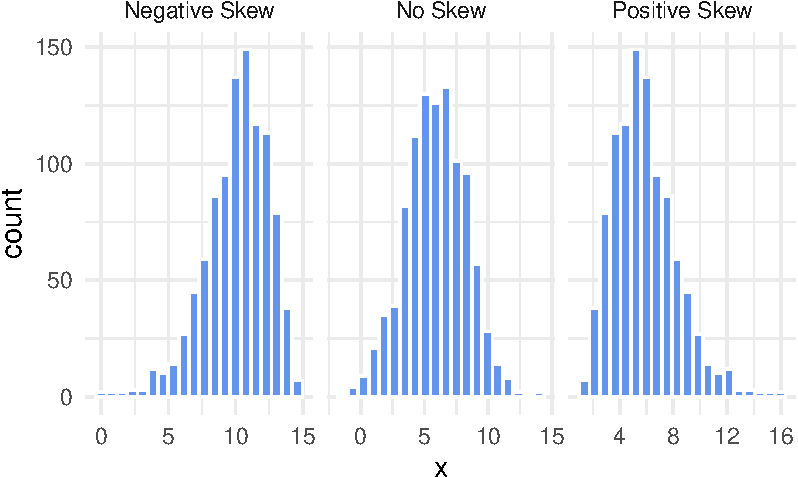
\includegraphics[keepaspectratio]{descriptives_files/figure-pdf/unnamed-chunk-20-1.pdf}}

\subsubsection{Kurtosis}\label{kurtosis}

The final measure that is sometimes referred to, though very rarely in
practice, is the~\textbf{\emph{kurtosis}}~of a data set. Put simply,
kurtosis is a measure of the ``pointiness'' of a data set.

\begin{Shaded}
\begin{Highlighting}[]
\FunctionTok{set.seed}\NormalTok{(}\DecValTok{123}\NormalTok{)}
\NormalTok{n }\OtherTok{\textless{}{-}} \DecValTok{1000}

\NormalTok{df }\OtherTok{\textless{}{-}} \FunctionTok{bind\_rows}\NormalTok{(}
  \FunctionTok{tibble}\NormalTok{(}\AttributeTok{x =} \FunctionTok{runif}\NormalTok{(n, }\SpecialCharTok{{-}}\FunctionTok{sqrt}\NormalTok{(}\DecValTok{3}\NormalTok{),  }\FunctionTok{sqrt}\NormalTok{(}\DecValTok{3}\NormalTok{)), }\AttributeTok{type =} \StringTok{"Platykurtic}\SpecialCharTok{\textbackslash{}n}\StringTok{(}\SpecialCharTok{\textbackslash{}"}\StringTok{too flat}\SpecialCharTok{\textbackslash{}"}\StringTok{)"}\NormalTok{),}
  \FunctionTok{tibble}\NormalTok{(}\AttributeTok{x =} \FunctionTok{rnorm}\NormalTok{(n),                      }\AttributeTok{type =} \StringTok{"Mesokurtic"}\NormalTok{),}
  \FunctionTok{tibble}\NormalTok{(}\AttributeTok{x =} \FunctionTok{rt}\NormalTok{(n, }\AttributeTok{df =} \DecValTok{3}\NormalTok{) }\SpecialCharTok{/} \FunctionTok{sd}\NormalTok{(}\FunctionTok{rt}\NormalTok{(n, }\AttributeTok{df =} \DecValTok{3}\NormalTok{)), }\AttributeTok{type =} \StringTok{"Leptokurtic}\SpecialCharTok{\textbackslash{}n}\StringTok{(}\SpecialCharTok{\textbackslash{}"}\StringTok{too pointy}\SpecialCharTok{\textbackslash{}"}\StringTok{)"}\NormalTok{)}
\NormalTok{) }\SpecialCharTok{\%\textgreater{}\%}
  \FunctionTok{mutate}\NormalTok{(}\AttributeTok{type =} \FunctionTok{factor}\NormalTok{(type, }\AttributeTok{levels =} \FunctionTok{c}\NormalTok{(}
    \StringTok{"Platykurtic}\SpecialCharTok{\textbackslash{}n}\StringTok{(}\SpecialCharTok{\textbackslash{}"}\StringTok{too flat}\SpecialCharTok{\textbackslash{}"}\StringTok{)"}\NormalTok{,}
    \StringTok{"Mesokurtic"}\NormalTok{,}
    \StringTok{"Leptokurtic}\SpecialCharTok{\textbackslash{}n}\StringTok{(}\SpecialCharTok{\textbackslash{}"}\StringTok{too pointy}\SpecialCharTok{\textbackslash{}"}\StringTok{)"}
\NormalTok{  )))}

\FunctionTok{ggplot}\NormalTok{(df, }\FunctionTok{aes}\NormalTok{(x)) }\SpecialCharTok{+}
  \FunctionTok{geom\_histogram}\NormalTok{(}\FunctionTok{aes}\NormalTok{(}\AttributeTok{y =} \FunctionTok{after\_stat}\NormalTok{(density)),}
                 \AttributeTok{bins =} \DecValTok{22}\NormalTok{, }\AttributeTok{fill =} \StringTok{"cornflowerblue"}\NormalTok{, }\AttributeTok{color =} \StringTok{"white"}\NormalTok{) }\SpecialCharTok{+}
  \FunctionTok{stat\_function}\NormalTok{(}\AttributeTok{fun =}\NormalTok{ dnorm, }\AttributeTok{linewidth =} \DecValTok{1}\NormalTok{) }\SpecialCharTok{+}
  \FunctionTok{facet\_wrap}\NormalTok{(}\SpecialCharTok{\textasciitilde{}}\NormalTok{ type, }\AttributeTok{nrow =} \DecValTok{1}\NormalTok{) }\SpecialCharTok{+}
  \FunctionTok{theme\_classic}\NormalTok{(}\AttributeTok{base\_size =} \DecValTok{14}\NormalTok{) }\SpecialCharTok{+}
  \FunctionTok{theme}\NormalTok{(}\AttributeTok{strip.background =} \FunctionTok{element\_blank}\NormalTok{())}
\end{Highlighting}
\end{Shaded}

\pandocbounded{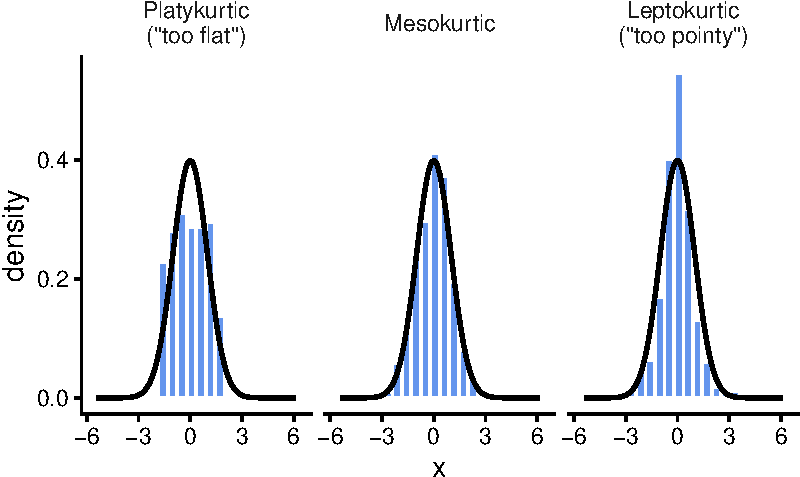
\includegraphics[keepaspectratio]{descriptives_files/figure-pdf/unnamed-chunk-21-1.pdf}}

\begin{center}\rule{0.5\linewidth}{0.5pt}\end{center}

\subsubsection{Moving Average}\label{moving-average}

Adding consecutive observations for a number of periods and dividing the
result by the number of periods included in the average.

\begin{Shaded}
\begin{Highlighting}[]
\FunctionTok{set.seed}\NormalTok{(}\DecValTok{123}\NormalTok{)}

\NormalTok{df }\OtherTok{\textless{}{-}} \FunctionTok{data.frame}\NormalTok{(}
  \AttributeTok{time =} \DecValTok{1}\SpecialCharTok{:}\DecValTok{30}\NormalTok{,}
  \AttributeTok{value =} \FunctionTok{cumsum}\NormalTok{(}\FunctionTok{rnorm}\NormalTok{(}\DecValTok{30}\NormalTok{))}
\NormalTok{)}

\NormalTok{df}\SpecialCharTok{$}\NormalTok{ma\_3 }\OtherTok{\textless{}{-}}\NormalTok{ stats}\SpecialCharTok{::}\FunctionTok{filter}\NormalTok{(df}\SpecialCharTok{$}\NormalTok{value, }\FunctionTok{rep}\NormalTok{(}\DecValTok{1}\SpecialCharTok{/}\DecValTok{3}\NormalTok{, }\DecValTok{3}\NormalTok{), }\AttributeTok{sides =} \DecValTok{2}\NormalTok{)}


\FunctionTok{library}\NormalTok{(ggplot2)}

\FunctionTok{ggplot}\NormalTok{(df, }\FunctionTok{aes}\NormalTok{(}\AttributeTok{x =}\NormalTok{ time)) }\SpecialCharTok{+}
  \FunctionTok{geom\_line}\NormalTok{(}\FunctionTok{aes}\NormalTok{(}\AttributeTok{y =}\NormalTok{ value), }\AttributeTok{alpha =} \FloatTok{0.6}\NormalTok{) }\SpecialCharTok{+}
  \FunctionTok{geom\_line}\NormalTok{(}\FunctionTok{aes}\NormalTok{(}\AttributeTok{y =}\NormalTok{ ma\_3), }\AttributeTok{linewidth =} \FloatTok{1.2}\NormalTok{) }\SpecialCharTok{+}
  \FunctionTok{theme\_classic}\NormalTok{(}\AttributeTok{base\_size =} \DecValTok{14}\NormalTok{) }\SpecialCharTok{+}
  \FunctionTok{labs}\NormalTok{(}
    \AttributeTok{title =} \StringTok{"Moving Average Smooths Short{-}Term Fluctuations"}\NormalTok{,}
    \AttributeTok{x =} \StringTok{"Time"}\NormalTok{,}
    \AttributeTok{y =} \StringTok{"Value"}
\NormalTok{  )}
\end{Highlighting}
\end{Shaded}

\pandocbounded{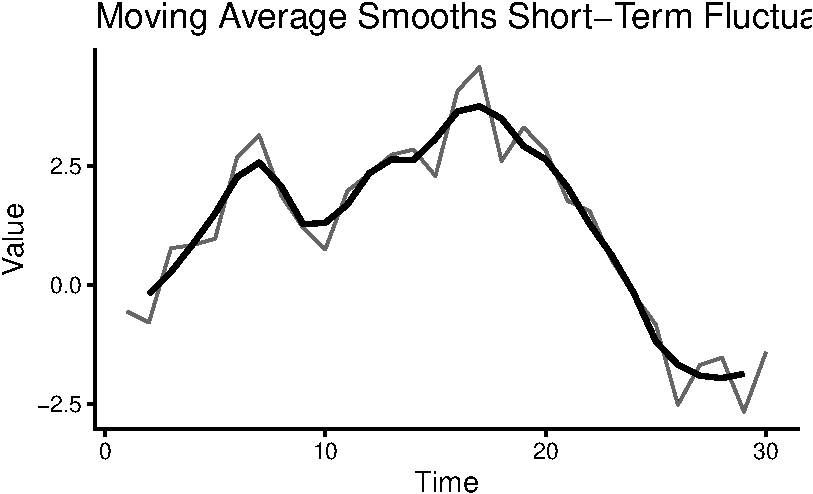
\includegraphics[keepaspectratio]{descriptives_files/figure-pdf/unnamed-chunk-22-1.pdf}}

\begin{center}\rule{0.5\linewidth}{0.5pt}\end{center}

\subsection{Dispersion}\label{dispersion}

\subsubsection{Range}\label{range}

\emph{The difference between the largest and smallest data values}

\begin{Shaded}
\begin{Highlighting}[]
\NormalTok{max\_mass }\OtherTok{\textless{}{-}} \FunctionTok{max}\NormalTok{(starwars}\SpecialCharTok{$}\NormalTok{mass, }\AttributeTok{na.rm =} \ConstantTok{TRUE}\NormalTok{)}
\NormalTok{min\_mass }\OtherTok{\textless{}{-}} \FunctionTok{min}\NormalTok{(starwars}\SpecialCharTok{$}\NormalTok{mass, }\AttributeTok{na.rm =} \ConstantTok{TRUE}\NormalTok{)}

\NormalTok{max\_mass}
\end{Highlighting}
\end{Shaded}

\begin{verbatim}
[1] 1358
\end{verbatim}

\begin{Shaded}
\begin{Highlighting}[]
\NormalTok{min\_mass}
\end{Highlighting}
\end{Shaded}

\begin{verbatim}
[1] 15
\end{verbatim}

\begin{Shaded}
\begin{Highlighting}[]
\FunctionTok{cat}\NormalTok{(}\StringTok{"["}\NormalTok{,min\_mass, }\StringTok{", "}\NormalTok{, max\_mass, }\StringTok{"]"}\NormalTok{)}
\end{Highlighting}
\end{Shaded}

\begin{verbatim}
[ 15 ,  1358 ]
\end{verbatim}

Or simply run the function\ldots{}

\begin{Shaded}
\begin{Highlighting}[]
\FunctionTok{range}\NormalTok{(starwars}\SpecialCharTok{$}\NormalTok{mass, }\AttributeTok{na.rm =} \ConstantTok{TRUE}\NormalTok{)}
\end{Highlighting}
\end{Shaded}

\begin{verbatim}
[1]   15 1358
\end{verbatim}

Although the range is the simplest way to quantify the notion of
``variability'', it's one of the worst.~If the data set has one or two
extremely bad values in it, we'd like our statistics not to be unduly
influenced by these cases.

\subsubsection{Variability}\label{variability}

The amount of individual observation or set of observations fluctuates
about the mean or center of set of data.

Deviation is distance that a value is from the mean.

\paragraph{Sample Variance}\label{sample-variance}

For each observation, calculate the distance from the mean. Square.
Then, sum. Divide by n-1.

\[s^2 = \frac{\sum (x_i - \bar{x})^2}{n - 1}\]

Imagine that we have the heights of 5 dogs, measured at their shoulder.

\[600mm, 470mm, 170mm, 430mm, 300mm\]

\begin{Shaded}
\begin{Highlighting}[]
\NormalTok{x }\OtherTok{\textless{}{-}} \FunctionTok{c}\NormalTok{(}\DecValTok{600}\NormalTok{, }\DecValTok{470}\NormalTok{, }\DecValTok{170}\NormalTok{, }\DecValTok{430}\NormalTok{, }\DecValTok{300}\NormalTok{)}
\end{Highlighting}
\end{Shaded}

If I was doing this by hand, I'll need to know the mean to use in the
formula.

\begin{Shaded}
\begin{Highlighting}[]
\NormalTok{xbar }\OtherTok{\textless{}{-}} \FunctionTok{mean}\NormalTok{(x)}
\end{Highlighting}
\end{Shaded}

Next, subtract the mean from each dog's height.

\begin{Shaded}
\begin{Highlighting}[]
\NormalTok{difference }\OtherTok{\textless{}{-}}\NormalTok{ x }\SpecialCharTok{{-}}\NormalTok{ xbar}
\NormalTok{difference}
\end{Highlighting}
\end{Shaded}

\begin{verbatim}
[1]  206   76 -224   36  -94
\end{verbatim}

Square it.

\begin{Shaded}
\begin{Highlighting}[]
\NormalTok{squared }\OtherTok{\textless{}{-}}\NormalTok{ (difference }\SpecialCharTok{*}\NormalTok{ difference)}
\NormalTok{squared}
\end{Highlighting}
\end{Shaded}

\begin{verbatim}
[1] 42436  5776 50176  1296  8836
\end{verbatim}

Sum it up.

\begin{Shaded}
\begin{Highlighting}[]
\NormalTok{summed\_up }\OtherTok{\textless{}{-}} \FunctionTok{sum}\NormalTok{(squared)}
\NormalTok{summed\_up}
\end{Highlighting}
\end{Shaded}

\begin{verbatim}
[1] 108520
\end{verbatim}

Divided by n - 1.

\begin{Shaded}
\begin{Highlighting}[]
\NormalTok{variance }\OtherTok{\textless{}{-}}\NormalTok{ summed\_up }\SpecialCharTok{/} \FunctionTok{length}\NormalTok{(x)}
\NormalTok{variance}
\end{Highlighting}
\end{Shaded}

\begin{verbatim}
[1] 21704
\end{verbatim}

\subsubsection{Mean Absolute Deviation
(MAD)}\label{mean-absolute-deviation-mad}

\[\mathrm{MAD} = \frac{\sum \lvert x_i - \bar{x} \rvert}{n}\]

One possibility would be to do everything using low level commands,
laboriously following the calculations above. However, that's pretty
tedious.

You'd end up with a series of commands that might look like this:

\begin{Shaded}
\begin{Highlighting}[]
\NormalTok{X }\OtherTok{\textless{}{-}} \FunctionTok{c}\NormalTok{(}\DecValTok{600}\NormalTok{, }\DecValTok{470}\NormalTok{, }\DecValTok{170}\NormalTok{, }\DecValTok{430}\NormalTok{, }\DecValTok{300}\NormalTok{)   }\CommentTok{\# enter the data}
\end{Highlighting}
\end{Shaded}

\begin{Shaded}
\begin{Highlighting}[]
\NormalTok{X.bar }\OtherTok{\textless{}{-}} \FunctionTok{mean}\NormalTok{( X )       }\CommentTok{\# step 1. the mean of the data}
\NormalTok{AD }\OtherTok{\textless{}{-}} \FunctionTok{abs}\NormalTok{( X }\SpecialCharTok{{-}}\NormalTok{ X.bar )   }\CommentTok{\# step 2. the absolute deviations from the mean}
\NormalTok{MAD }\OtherTok{\textless{}{-}} \FunctionTok{mean}\NormalTok{( AD )        }\CommentTok{\# step 3. the mean absolute deviations}
\FunctionTok{print}\NormalTok{( MAD )             }\CommentTok{\# print the results}
\end{Highlighting}
\end{Shaded}

\begin{verbatim}
[1] 127.2
\end{verbatim}

Each of those commands is pretty simple, but there's just too many of
them. And because I find that to be too much typing,
the~\texttt{lsr}~package has a very simple function
called~\texttt{aad()}~that does the calculations for you. If we apply
the~\texttt{aad()}~function to our data, we get this:

\begin{Shaded}
\begin{Highlighting}[]
\NormalTok{lsr}\SpecialCharTok{::}\FunctionTok{aad}\NormalTok{(X)}
\end{Highlighting}
\end{Shaded}

\begin{verbatim}
[1] 127.2
\end{verbatim}

No suprises there.

\subsubsection{Standard Deviation}\label{standard-deviation}

Simply take the square root of the variance.

\begin{Shaded}
\begin{Highlighting}[]
\NormalTok{SD }\OtherTok{\textless{}{-}} \FunctionTok{sqrt}\NormalTok{(variance)}
\NormalTok{SD}
\end{Highlighting}
\end{Shaded}

\begin{verbatim}
[1] 147.3228
\end{verbatim}

For population SD, use N. For sample SD use n-1.

\paragraph{Why use square
differences?}\label{why-use-square-differences}

If we just add up the differences from the mean the negatives cancel the
positives:

\[\frac{4 + 4 - 4 - 4}{4} = 0\]

\pandocbounded{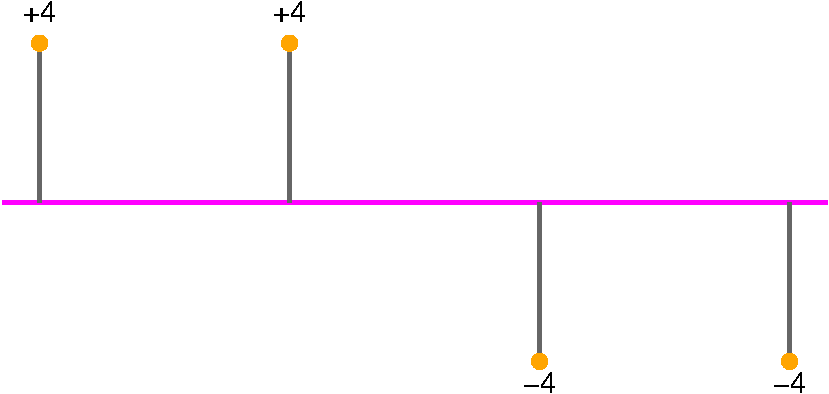
\includegraphics[keepaspectratio]{descriptives_files/figure-pdf/unnamed-chunk-36-1.pdf}}

What about absolute values? That's MAD.

\[\frac{|4| + |4| + |-4| + |-4|}{4}= \frac{4 + 4 + 4 + 4}{4}= 4\]

Not to bad, but\ldots. it does not always work out. Consider this:

\[\frac{|7| + |1| + |-6| + |-2|}{4}= \frac{7 + 1 + 6 + 2}{4}= 4\]

Clearly more spread than the first one, but the same results.

\begin{Shaded}
\begin{Highlighting}[]
\NormalTok{df7 }\OtherTok{\textless{}{-}} \FunctionTok{data.frame}\NormalTok{(}
  \AttributeTok{x =} \FunctionTok{c}\NormalTok{(}\DecValTok{1}\NormalTok{, }\DecValTok{2}\NormalTok{, }\DecValTok{3}\NormalTok{, }\DecValTok{4}\NormalTok{),}
  \AttributeTok{y =} \FunctionTok{c}\NormalTok{(}\DecValTok{7}\NormalTok{, }\DecValTok{1}\NormalTok{, }\SpecialCharTok{{-}}\DecValTok{6}\NormalTok{, }\SpecialCharTok{{-}}\DecValTok{2}\NormalTok{),}
  \AttributeTok{label =} \FunctionTok{c}\NormalTok{(}\StringTok{"+7"}\NormalTok{, }\StringTok{"+1"}\NormalTok{, }\StringTok{"{-}6"}\NormalTok{, }\StringTok{"{-}2"}\NormalTok{)}
\NormalTok{)}

\FunctionTok{ggplot}\NormalTok{(df7, }\FunctionTok{aes}\NormalTok{(}\AttributeTok{x =}\NormalTok{ x, }\AttributeTok{y =}\NormalTok{ y)) }\SpecialCharTok{+}
  \FunctionTok{geom\_hline}\NormalTok{(}\AttributeTok{yintercept =} \DecValTok{0}\NormalTok{, }\AttributeTok{color =} \StringTok{"magenta"}\NormalTok{, }\AttributeTok{linewidth =} \DecValTok{1}\NormalTok{) }\SpecialCharTok{+}
  \FunctionTok{geom\_segment}\NormalTok{(}\FunctionTok{aes}\NormalTok{(}\AttributeTok{xend =}\NormalTok{ x, }\AttributeTok{y =} \DecValTok{0}\NormalTok{, }\AttributeTok{yend =}\NormalTok{ y),}
               \AttributeTok{linewidth =} \DecValTok{1}\NormalTok{, }\AttributeTok{color =} \StringTok{"gray40"}\NormalTok{) }\SpecialCharTok{+}
  \FunctionTok{geom\_point}\NormalTok{(}\AttributeTok{size =} \DecValTok{3}\NormalTok{, }\AttributeTok{color =} \StringTok{"orange"}\NormalTok{) }\SpecialCharTok{+}
  \FunctionTok{geom\_text}\NormalTok{(}
    \FunctionTok{aes}\NormalTok{(}\AttributeTok{label =}\NormalTok{ label),}
    \AttributeTok{vjust =} \FunctionTok{ifelse}\NormalTok{(df7}\SpecialCharTok{$}\NormalTok{y }\SpecialCharTok{\textgreater{}} \DecValTok{0}\NormalTok{, }\SpecialCharTok{{-}}\FloatTok{0.8}\NormalTok{, }\FloatTok{1.3}\NormalTok{),}
    \AttributeTok{size =} \DecValTok{5}
\NormalTok{  ) }\SpecialCharTok{+}
  \FunctionTok{scale\_y\_continuous}\NormalTok{(}
    \AttributeTok{limits =} \FunctionTok{c}\NormalTok{(}\FunctionTok{min}\NormalTok{(df7}\SpecialCharTok{$}\NormalTok{y) }\SpecialCharTok{{-}} \DecValTok{2}\NormalTok{, }\FunctionTok{max}\NormalTok{(df7}\SpecialCharTok{$}\NormalTok{y) }\SpecialCharTok{+} \DecValTok{2}\NormalTok{)}
\NormalTok{  ) }\SpecialCharTok{+}
  \FunctionTok{theme\_void}\NormalTok{()}
\end{Highlighting}
\end{Shaded}

\pandocbounded{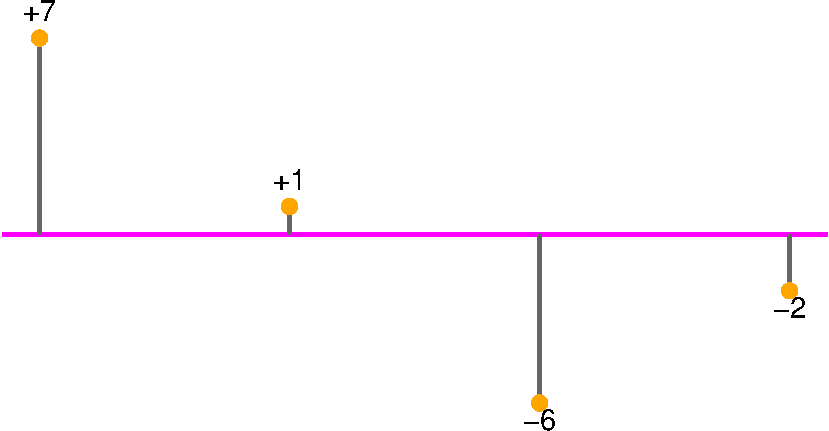
\includegraphics[keepaspectratio]{descriptives_files/figure-pdf/unnamed-chunk-37-1.pdf}}

So lets try to square them and then take the square root at the end.

\[\sqrt{\frac{4^2 + 4^2 + (-4)^2 + (-4)^2}{4}}= \sqrt{\frac{64}{4}}= 4\]

\[\sqrt{\frac{7^2 + 1^2 + (-6)^2 + (-2)^2}{4}}= \sqrt{\frac{90}{4}}= 4.74\]

Success! The standard deviation is bigger when the data is more spread
out. Hence, why we use this approach.

\subsection{Empirical Rule}\label{empirical-rule}

The variability of a set of measurements for a \textbf{bell-shaped
distribution}. Most values cluster around the mean.

\begin{itemize}
\tightlist
\item
  About \textbf{68\%} of the data fall within \textbf{1} standard
  deviation of the mean
\end{itemize}

\begin{itemize}
\tightlist
\item
  About \textbf{95\%} of the data fall within \textbf{2} standard
  deviations of the mean
\end{itemize}

\begin{itemize}
\tightlist
\item
  About \textbf{99.7\%} of the data fall within \textbf{3} standard
  deviations of the mean
\end{itemize}

\begin{Shaded}
\begin{Highlighting}[]
\FunctionTok{set.seed}\NormalTok{(}\DecValTok{123}\NormalTok{)}
\NormalTok{x }\OtherTok{\textless{}{-}} \FunctionTok{rnorm}\NormalTok{(}\DecValTok{10000}\NormalTok{)}
\NormalTok{df }\OtherTok{\textless{}{-}} \FunctionTok{data.frame}\NormalTok{(x)}

\NormalTok{mu }\OtherTok{\textless{}{-}} \FunctionTok{mean}\NormalTok{(df}\SpecialCharTok{$}\NormalTok{x)}
\NormalTok{sdx }\OtherTok{\textless{}{-}} \FunctionTok{sd}\NormalTok{(df}\SpecialCharTok{$}\NormalTok{x)}

\FunctionTok{ggplot}\NormalTok{(df, }\FunctionTok{aes}\NormalTok{(x)) }\SpecialCharTok{+}
  \FunctionTok{stat\_function}\NormalTok{(}\AttributeTok{fun =}\NormalTok{ dnorm, }\AttributeTok{args =} \FunctionTok{list}\NormalTok{(}\AttributeTok{mean =}\NormalTok{ mu, }\AttributeTok{sd =}\NormalTok{ sdx)) }\SpecialCharTok{+}

  \CommentTok{\# 68\%}
  \FunctionTok{stat\_function}\NormalTok{(}
    \AttributeTok{fun =}\NormalTok{ dnorm,}
    \AttributeTok{args =} \FunctionTok{list}\NormalTok{(}\AttributeTok{mean =}\NormalTok{ mu, }\AttributeTok{sd =}\NormalTok{ sdx),}
    \AttributeTok{xlim =} \FunctionTok{c}\NormalTok{(mu }\SpecialCharTok{{-}}\NormalTok{ sdx, mu }\SpecialCharTok{+}\NormalTok{ sdx),}
    \AttributeTok{geom =} \StringTok{"area"}\NormalTok{,}
    \AttributeTok{alpha =} \FloatTok{0.4}
\NormalTok{  ) }\SpecialCharTok{+}

  \CommentTok{\# 95\%}
  \FunctionTok{stat\_function}\NormalTok{(}
    \AttributeTok{fun =}\NormalTok{ dnorm,}
    \AttributeTok{args =} \FunctionTok{list}\NormalTok{(}\AttributeTok{mean =}\NormalTok{ mu, }\AttributeTok{sd =}\NormalTok{ sdx),}
    \AttributeTok{xlim =} \FunctionTok{c}\NormalTok{(mu }\SpecialCharTok{{-}} \DecValTok{2} \SpecialCharTok{*}\NormalTok{ sdx, mu }\SpecialCharTok{+} \DecValTok{2} \SpecialCharTok{*}\NormalTok{ sdx),}
    \AttributeTok{geom =} \StringTok{"area"}\NormalTok{,}
    \AttributeTok{alpha =} \FloatTok{0.25}
\NormalTok{  ) }\SpecialCharTok{+}

  \CommentTok{\# 99.7\%}
  \FunctionTok{stat\_function}\NormalTok{(}
    \AttributeTok{fun =}\NormalTok{ dnorm,}
    \AttributeTok{args =} \FunctionTok{list}\NormalTok{(}\AttributeTok{mean =}\NormalTok{ mu, }\AttributeTok{sd =}\NormalTok{ sdx),}
    \AttributeTok{xlim =} \FunctionTok{c}\NormalTok{(mu }\SpecialCharTok{{-}} \DecValTok{3} \SpecialCharTok{*}\NormalTok{ sdx, mu }\SpecialCharTok{+} \DecValTok{3} \SpecialCharTok{*}\NormalTok{ sdx),}
    \AttributeTok{geom =} \StringTok{"area"}\NormalTok{,}
    \AttributeTok{alpha =} \FloatTok{0.15}
\NormalTok{  ) }\SpecialCharTok{+}

  \FunctionTok{theme\_classic}\NormalTok{(}\AttributeTok{base\_size =} \DecValTok{14}\NormalTok{) }\SpecialCharTok{+}
  \FunctionTok{labs}\NormalTok{(}
    \AttributeTok{title =} \StringTok{"Empirical Rule (68–95–99.7)"}\NormalTok{,}
    \AttributeTok{x =} \StringTok{"Mean"}\NormalTok{,}
    \AttributeTok{y =} \StringTok{"Density"}\NormalTok{) }\SpecialCharTok{+} 
  \FunctionTok{scale\_x\_continuous}\NormalTok{(}
  \AttributeTok{breaks =}\NormalTok{ mu }\SpecialCharTok{+}\NormalTok{ (}\SpecialCharTok{{-}}\DecValTok{3}\SpecialCharTok{:}\DecValTok{3}\NormalTok{) }\SpecialCharTok{*}\NormalTok{ sdx,}
  \AttributeTok{labels =} \FunctionTok{c}\NormalTok{(}\StringTok{"{-}3 SD"}\NormalTok{, }\StringTok{"{-}2 SD"}\NormalTok{, }\StringTok{"{-}1 SD"}\NormalTok{, }\StringTok{"0"}\NormalTok{, }\StringTok{"+1 SD"}\NormalTok{, }\StringTok{"+2 SD"}\NormalTok{, }\StringTok{"+3 SD"}\NormalTok{)}
\NormalTok{)}
\end{Highlighting}
\end{Shaded}

\pandocbounded{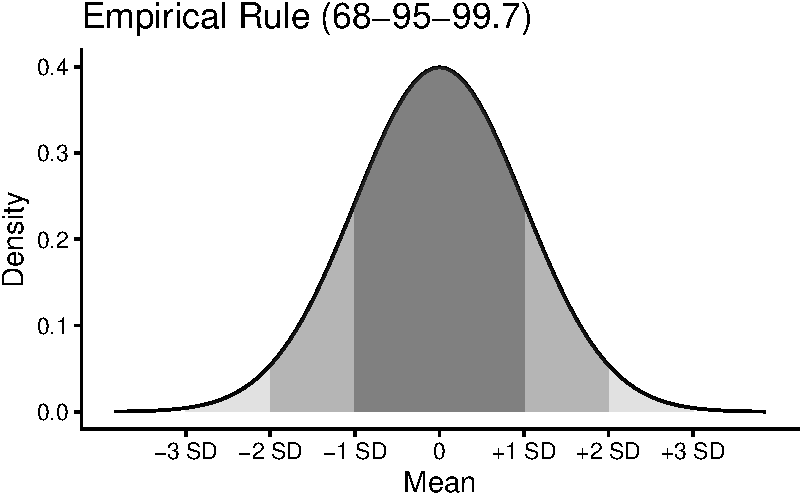
\includegraphics[keepaspectratio]{descriptives_files/figure-pdf/unnamed-chunk-38-1.pdf}}

\subsubsection{Chebyshev's Theorem}\label{chebyshevs-theorem}

General rule that describes the variability of any set of data
regardless of the shape of its distribution.

\[1 - \frac{1}{k^2}, \quad \text{for } k > 1\]

\subsection{Coefficient of Variation}\label{coefficient-of-variation}

Compares the variation in data sets.

\[\mathrm{CV} = \left( \frac{s}{\bar{x}} \cdot 100 \right)\%\]

\subsection{Additional Functions}\label{additional-functions}

\begin{Shaded}
\begin{Highlighting}[]
\FunctionTok{summary}\NormalTok{(starwars}\SpecialCharTok{$}\NormalTok{height)}
\end{Highlighting}
\end{Shaded}

\begin{verbatim}
   Min. 1st Qu.  Median    Mean 3rd Qu.    Max.     NAs 
   66.0   167.0   180.0   174.6   191.0   264.0       6 
\end{verbatim}

\begin{Shaded}
\begin{Highlighting}[]
\NormalTok{psych}\SpecialCharTok{::}\FunctionTok{describe}\NormalTok{(starwars}\SpecialCharTok{$}\NormalTok{height)}
\end{Highlighting}
\end{Shaded}

\begin{verbatim}
   vars  n  mean    sd median trimmed   mad min max range  skew kurtosis   se
X1    1 81 174.6 34.77    180  178.48 17.79  66 264   198 -1.05      1.8 3.86
\end{verbatim}

Acknowledgements: learningstatisticswithR




\end{document}
